\documentclass[a4paper]{article}
\usepackage{graphicx}
\usepackage{epstopdf}
\usepackage{mcode}
\usepackage{style}
\usepackage{float}
\title{Laboration i Komponentfysik\\ Den bipolära transistorn}

\author{Alexander Najafi \\ Linus Hellman}

\date{2014-05-10}

\begin{document}

\maketitle
\thispagestyle{empty}
\newpage

\tableofcontents
\newpage
\section{Introduction}
The purpose of this lab is to gain a better understanding of the bipolar transistor characteristics. By altering the different potentials over the three sections of the transistor we hope to establish a connection between them and in that way learn to understand it. The lab mainly consists in three parts, measuring the capacitor in a pn-junction, measuring the current through a pn-junction and measuring the currents through a bipolar npn-transistor.

In the first part we are studying the capacitor in the pn-junction. The total capacitance that is found in a pn-junction actually consists of capacitors from two different origins, one is called junction capacity and the other one is called diffusion capacity. The junction capacity exist because of that the depletion area has a very high resistance so that when the n and p sections has voltage difference the junction can be seen as a capacitor. The second capacitor origins in the neutral part of the p-doped section. When the pn-junction is forward biased the the 

\section{Result}
\subsection{PN junction UI}
The following graph was plotted for the PN junction U-I characteristics. See the measured data in the appendix together with the matlab-code. 
\begin{figure}[H]
	\centering
	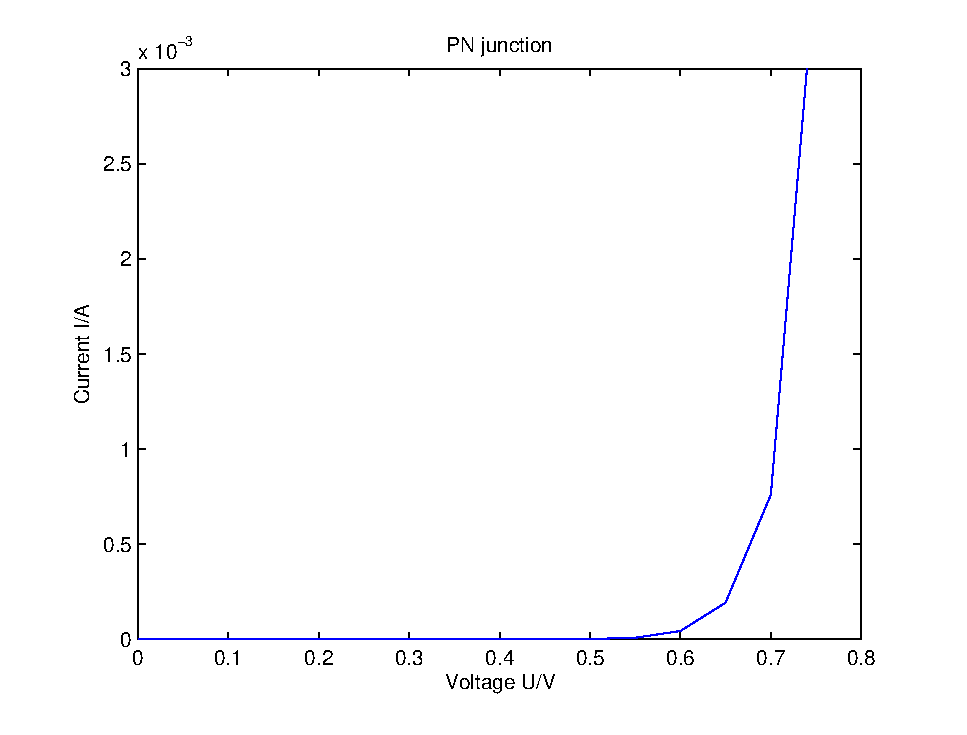
\includegraphics[width=0.7\textwidth]{pn_ui.eps}
	\caption{U-I characterstics for the PN junction.}	
	\label{pn_ui}
\end{figure}

\subsection{PN junction capacitance}
The following graph was plotted using the measured data in the appendix for the capacitance in the PN junction. See appendix for values and matlab-code. 
\begin{figure}[H]
	\centering
	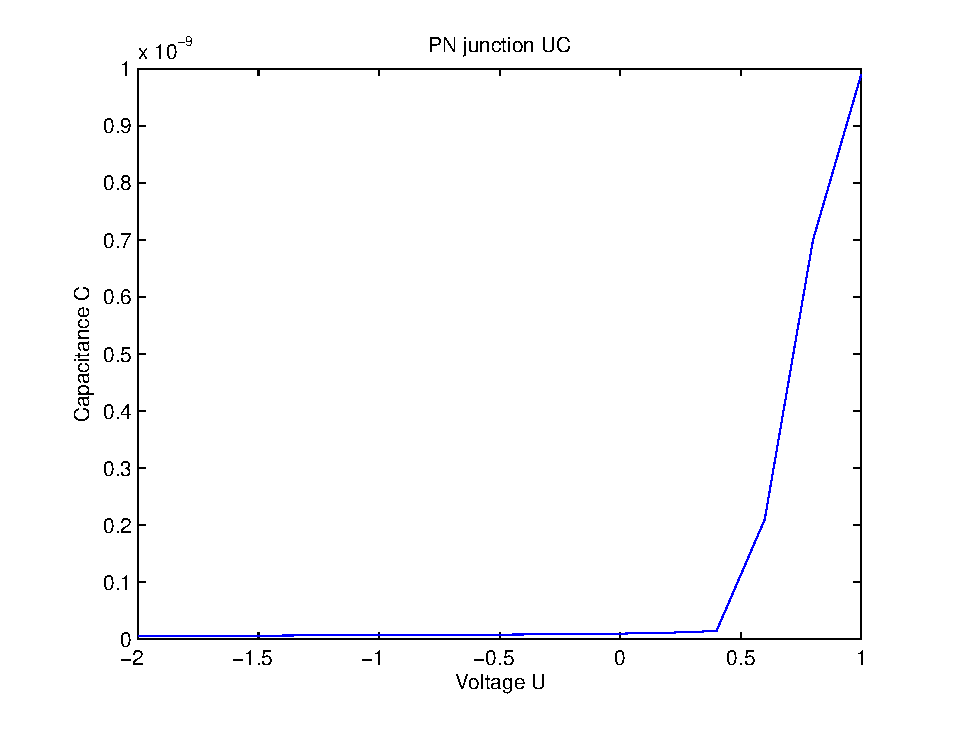
\includegraphics[width=0.7\textwidth]{pn_cap.eps}
	\caption{C-U characterstics for the PN junction.}	
	\label{pn_cap}
\end{figure}

\subsection{NPN transistor}
The following graphs were plotted for the current in the npn transistor. The early voltage was calculated to 34V using matlab. See the appendix for values and matlab-code.
\begin{figure}[H]
	\centering
	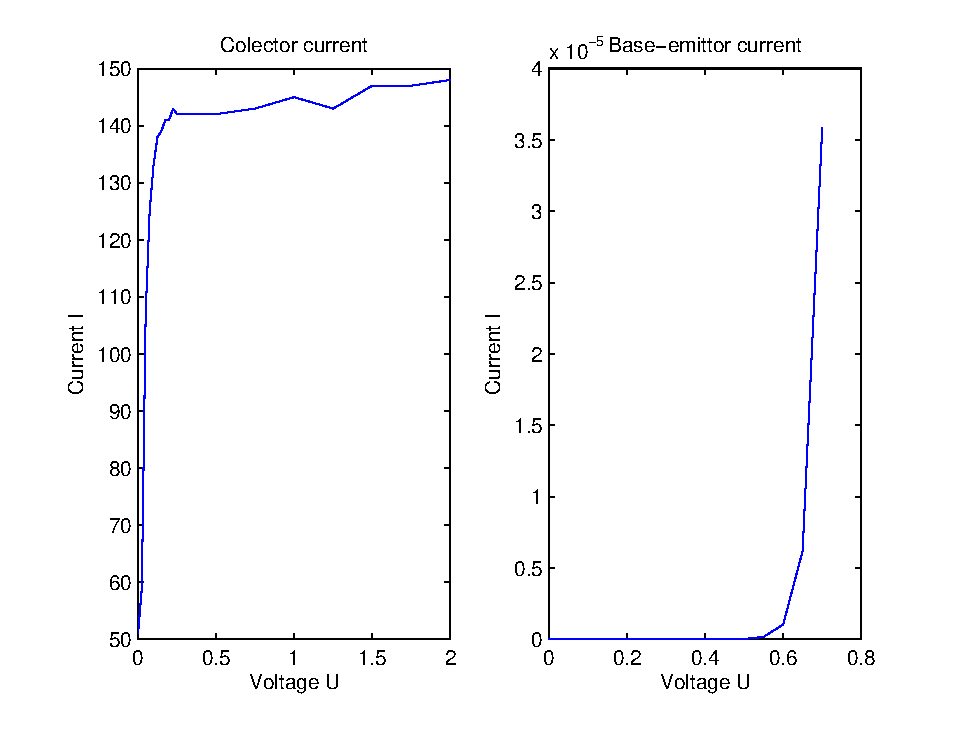
\includegraphics[width=0.85\textwidth]{npn.eps}
	\caption{Voltage to current characteristics for the NPN transistor. The collector current to the left and the base-emittor current to the right.}	
	\label{npn}
\end{figure}

\newpage
\section{Analysis of the result}
\subsection{NPN transistor}
As you can see to the left in figure \ref{npn} an increasing voltage from zero to about 0.25 volts results in a substantially increase in the collector current. The current does'nt increase to infinity and beyond though. The steep increase stops since there is no more electrons that can diffuse from the emittor through the base to the collector.

To calculate the early voltage a linear function was aproximated to the eleven largest values that were measured. To find the aproximation function $p(U) = ax + b$ polyfit was used in matlab (see appendix). Using the function and calculating $p(U) = 0 => x = \frac{b}{a}$ the earlyvoltage was found to be $\frac{139,9}{4,1} \approx 34V$.

\newpage
\appendix
\section{Matlab code}
\subsection{PN junction UI}
\lstinputlisting{pn_current.m}
\subsection{PN junction capacitance}
\lstinputlisting{pn_cap.m}
\subsection{NPN current}
\lstinputlisting{npn.m}

\end{document}
